\chapter{Algoritmi di sincronizzazione distribuiti}
Il modello a scambio di messaggi è la naturale astrazione di un sistema distribuito, nel quale processi distinti eseguono su nodi fisicamente separati e collegati tra loro attraverso una rete.

Caratteristiche sistemi distribuiti:
\begin{itemize}
    \item concorrenza/parallelismo delle attività dai nodi
    \item assenza di risorse condivise tra nodi
    \item assenza di un clock globale
    \item possibilità di malfunzionamenti indipendenti
    \begin{itemize}
        \item nei nodi (crash, attacchi...)
        \item nella rete di comunicazione
    \end{itemize}
\end{itemize}

Le proprietà desiderabili in sistemi di questo tipo:
\begin{itemize}
    \item \textbf{scalabilità}: le prestazioni dovrebbero aumentare al crescere del numero di nodi utilizzati
    \item \textbf{tolleranza ai guasti}: capacità di funzionare anche in presenza di guasti
\end{itemize}

\subsection{Prestazioni}
Un indicatore per misurare le prestazioni di un sistema parallelo è dato dallo \textbf{speedup}.

Ipotizzando che un'applicazione possa essere eseguita su un numero variabile di nodi, lo speedup è una funzione del numero di nodi.
\begin{equation*}
\texttt{speedup(n) = tempo(1) / tempo(n)}
\end{equation*}

\begin{figure}[H]
    \centering
    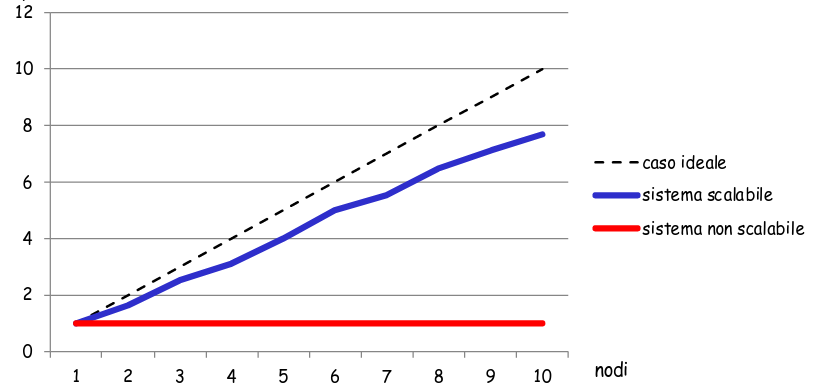
\includegraphics[width=0.6\textwidth]{/home/riccardoob/appunti/sistemi_operativi/images/52.png}
\end{figure}

Il grafico traccia la relazione tra speedup e numero di nodi n, lo speedup ideale è
\begin{equation*}
\texttt{speedup(n) = tempo(1) / tempo(n) = n}
\end{equation*}

\subsection{Tolleranza ai guasti}
Un sistema distribuito tollerante ai guasti riesce a erogare i propri servizi anche in presenza di guasti su uno o più nodi.

Tipi di guasti:
\begin{itemize}
    \item transiente
    \item intermittente
    \item persistente
\end{itemize}

La tolleranza ai guasti può essere conseguita con tecniche di \textbf{ridondanza}, vengono mantenute più istanze degli stessi componenti, in modo da poter rimpiazzare l'elemento guasto con un elemento equivalente.

É necessario prevedere meccanismi per
\begin{itemize}
    \item \textbf{rilevazione} dei guasti (\textit{fault detection})
    \item \textbf{ripristino} del sistema dopo ogni guasto rilevato (\textit{recovery})
\end{itemize}

\subsection{Algoritmi di sincronizzazione}
Come nel modello a memoria comune, anche nel modello a scambio di messaggi è necessario prevedere algoritmi che permettano la sincronizzazione tra processi concorrenti, per risolvere eventuali problematiche.

Ad esempio:
\begin{itemize}
    \item \textbf{timing}: sincronizzazione dei clock e tempo logico
    \item \textbf{mutua esclusione} distribuita
    \item elezione di \textbf{coordinatori} in gruppi di processi
\end{itemize}

É desiderabile che questi algoritmi godano delle proprietà di scalabilità e tolleranza ai guasti.

\section{Algoritmi per la gestione del tempo}

\subsection{Tempo nei sistemi distribuiti}
In un sistema distribuito, ogni nodo è dotato di un proprio orologio, se due orologi locali a due nodi non sono sincronizzati, è possibile che se un evento \texttt{e2} accade nel nodo \texttt{N2} dopo un altro evento \texttt{e1} nel nodo \texttt{N1}, ad \texttt{e2} sia associato un istante temporale precedente quello di \texttt{e1}.

In applicazioni distribuite può essere necessario avere un \textbf{unico riferimento temporale}, condiviso da tutti i partecipanti.

Realizzabile con:
\begin{itemize}
    \item un \textbf{orologio fisico universale}: a questo scopo vengono utilizzati degli algoritmi di sincronizzazione dei nodi del sistema (algoritmo di Berkley, algoritmo di Cristian) che garantiscono che il tempo misurato da ogni clock su ogni nodo sia lo stesso
    \item un \textbf{orologio logico}, che permetta di associare a ogni evento un istante logico coerente con l'ordine in cui essi si verificano
\end{itemize}

\subsection{Orologi logici}

\subsubsection{Relazione di precedenza tra eventi, Happened Before ->}
\begin{itemize}
    \item se \texttt{a} e \texttt{b} sono eventi in uno stesso processo e \texttt{a} si verifica prima di \texttt{b}: \texttt{a->b}
    \item se \texttt{a} è l'evento di \textbf{invio di un messaggio} e \texttt{b} è l'evento di \textbf{ricezione} dello stesso messaggio: \texttt{a->b}
    \item se \texttt{a->b} e \texttt{b->c} allora \texttt{a->c}
\end{itemize}

Data una coppia di eventi \texttt{(a,b)} sono possibili tre casi
\begin{itemize}
    \item \texttt{a->b}
    \item \texttt{b->a}
    \item \texttt{a} e \texttt{b} non sono legati dalla relazione \textbf{HB}, ovvero sono concorrenti
\end{itemize}

Assumendo che ad ogni evento venga associato un \textbf{timestamp} \texttt{C(e)}, si vuole definire un modo per misurare il concetto di tempo tale per cui ad ogni evento \texttt{a} possiamo associare un timetamp \texttt{C(a)} sul quale tutti i processi sono d'accordo.

I timestamp devono soddisfare la seguente proprietà
\begin{equation*}
\text{se }\texttt{a->b}\text{ allora }\texttt{C(a) < C(b)}
\end{equation*}

\subsubsection{Algoritmo di Lamport}
Per garantire il rispetto della proprietà, ogni processo \texttt{P}$_i$ gestisce localmente un \textbf{contatore} del tempo logico \texttt{C}$_i$, che viene gestito nel modo seguente:
\begin{itemize}
    \item ogni nuovo evento all'interno di \texttt{P}$_i$ provoca un incremento del valore di \texttt{C}$_i$: \texttt{C}$_i$ = \texttt{C}$_i$ + 1
    \item ogni volta che \texttt{P}$_i$ invia un messaggio \texttt{m}, il contatore \texttt{C}$_i$ viene incrementato: \texttt{C}$_i$ = \texttt{C}$_i$ + 1 e successivamente al messaggio viene associato il timestamp \texttt{C}$_i$: \texttt{ts(m)} = \texttt{C}$_i$
    \item quando un processo \texttt{P}$_j$ riceve un messaggio \texttt{m}, assegna al proprio contatore \texttt{C}$_j$ un valore uguale al massimo tra \texttt{C}$_j$ e \texttt{ts(m)}: \texttt{C}$_j$ = \texttt{max\{}\texttt{C}$_j$, \texttt{ts(m)\}} e successivamente lo incrementa di 1: \texttt{C}$_j$ = \texttt{C}$_j$ + 1
\end{itemize}

\subsubsection{Esempio}
Consideriamo tre processi in esecuzione su tre nodi, ognuno con il proprio clock (frequenze diverse):
\begin{figure}[H]
    \centering
    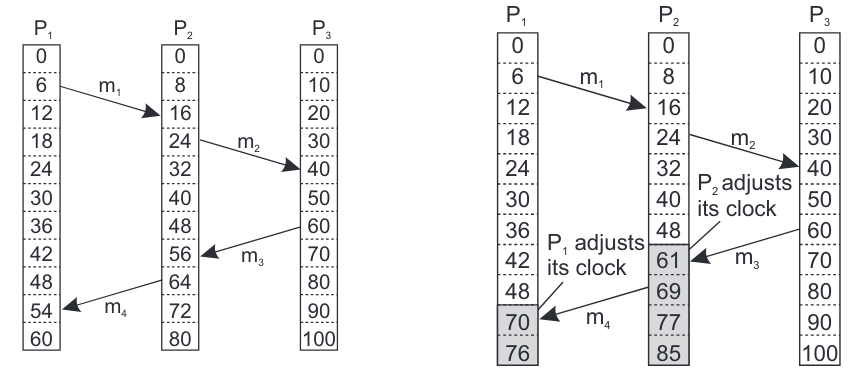
\includegraphics[width=0.6\textwidth]{/home/riccardoob/appunti/sistemi_operativi/images/53.png}
\end{figure}

\subsubsection{Lamport: aggiornamenti degli orologi}
Nei sistemi distribuiti, l'algoritmo di Lamport viene generalmente eseguito da uno strato di software (\textit{middleware)} che interfaccia i processi alla rete: i processi vedono solo il tempo logico.

\begin{figure}[H]
    \centering
    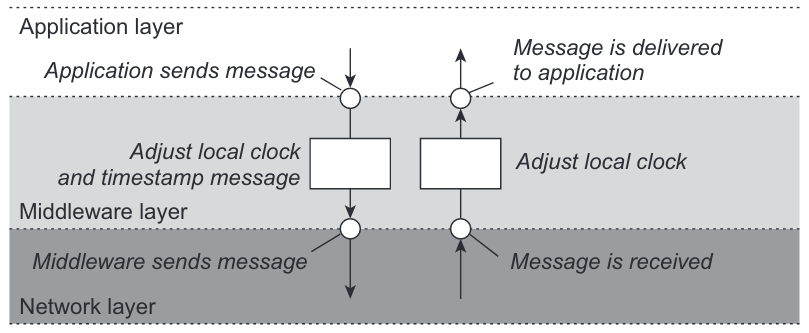
\includegraphics[width=0.6\textwidth]{/home/riccardoob/appunti/sistemi_operativi/images/54.png}
\end{figure}

\section{Mutua esclusione in sistemi distribuiti}
























































